% interactcadsample.tex
% v1.03 - April 2017

\documentclass[]{interact}

\usepackage{epstopdf}% To incorporate .eps illustrations using PDFLaTeX, etc.
\usepackage{subfigure}% Support for small, `sub' figures and tables
%\usepackage[nolists,tablesfirst]{endfloat}% To `separate' figures and tables from text if required

\usepackage{natbib}% Citation support using natbib.sty
\bibpunct[, ]{(}{)}{;}{a}{}{,}% Citation support using natbib.sty
\renewcommand\bibfont{\fontsize{10}{12}\selectfont}% Bibliography support using natbib.sty

\theoremstyle{plain}% Theorem-like structures provided by amsthm.sty
\newtheorem{theorem}{Theorem}[section]
\newtheorem{lemma}[theorem]{Lemma}
\newtheorem{corollary}[theorem]{Corollary}
\newtheorem{proposition}[theorem]{Proposition}

\theoremstyle{definition}
\newtheorem{definition}[theorem]{Definition}
\newtheorem{example}[theorem]{Example}

\theoremstyle{remark}
\newtheorem{remark}{Remark}
\newtheorem{notation}{Notation}

% see https://stackoverflow.com/a/47122900

% Pandoc citation processing

\usepackage{hyperref}
\usepackage[utf8]{inputenc}
\def\tightlist{}

\begin{document}

\articletype{}

\title{A manuscript about rivers}


\author{\name{Michael Dumelle$^{a}$}
\affil{$^{a}$United States Environmental Protection Agency - 200 SW 35th St,
Corvallis, OR, 97333}
}

\thanks{CONTACT Michael Dumelle. Email: \href{mailto:Dumelle.Michael@epa.gov}{\nolinkurl{Dumelle.Michael@epa.gov}}}

\maketitle

\begin{abstract}
This abstract about rivers secretly describes that this document serves
as a template for authors who are preparing a manuscript for a Taylor \&
Francis journal using the \LaTeX~document preparation system and the
\texttt{interact} class file, which is available via selected journals'
home pages on the Taylor \& Francis website.
\end{abstract}

\begin{keywords}
River; Length; Discharge
\end{keywords}

\hypertarget{intro}{%
\section{Introduction}\label{intro}}

This is my introduction about rivers. Next we talk about the background,
which I refer to here as Section \ref{background}.

\hypertarget{background}{%
\section{Background}\label{background}}

Rivers are neat. We wanted to study river length and discharge. Next we
give subsections discussing both.

\hypertarget{subsec:length}{%
\subsection{Length}\label{subsec:length}}

This is where I talk about river length.

\hypertarget{subsec:discharge}{%
\subsection{Discharge}\label{subsec:discharge}}

This is where I talk about river discharge.

\hypertarget{sec:methods}{%
\section{Methods}\label{sec:methods}}

This is where I talk about methods. It may include an equation like this
one defining a mean \begin{equation}\label{eq:mean}
  \bar{x} = \frac{1}{n}\sum_{i = 1}^n x_i
\end{equation} I can refer to that equation as Equation \ref{eq:mean}.

\hypertarget{sec:analysis}{%
\section{Analysis}\label{sec:analysis}}

\begin{table}[ht]
\centering
\begin{tabular}{rrrr}
  \hline
 & Colorado & Columbia & Canadian \\ 
  \hline
length & 2330.00 & 2000.00 & 1458.00 \\ 
  discharge & 40.00 & 7730.00 & 174.00 \\ 
   \hline
\end{tabular}
\caption{Rivers whose names start with C} 
\label{tab:rivers_C}
\end{table}
\begin{table}[ht]
\centering
\begin{tabular}{rlrr}
  \hline
 & pattern & length\_min & discharge\_min \\ 
  \hline
1 & C & 1458.00 & 40.00 \\ 
   \hline
\end{tabular}
\caption{Length and discharge minimums for rives whose names start with C} 
\label{tab:rivers_min}
\end{table}

The length minimum in Table \ref{tab:rivers_min} is 1458 kilometers.
Further exploring the data, we present a plot of river length vs
discharge in Figure \ref{fig:rivers}.

\begin{figure}

{\centering 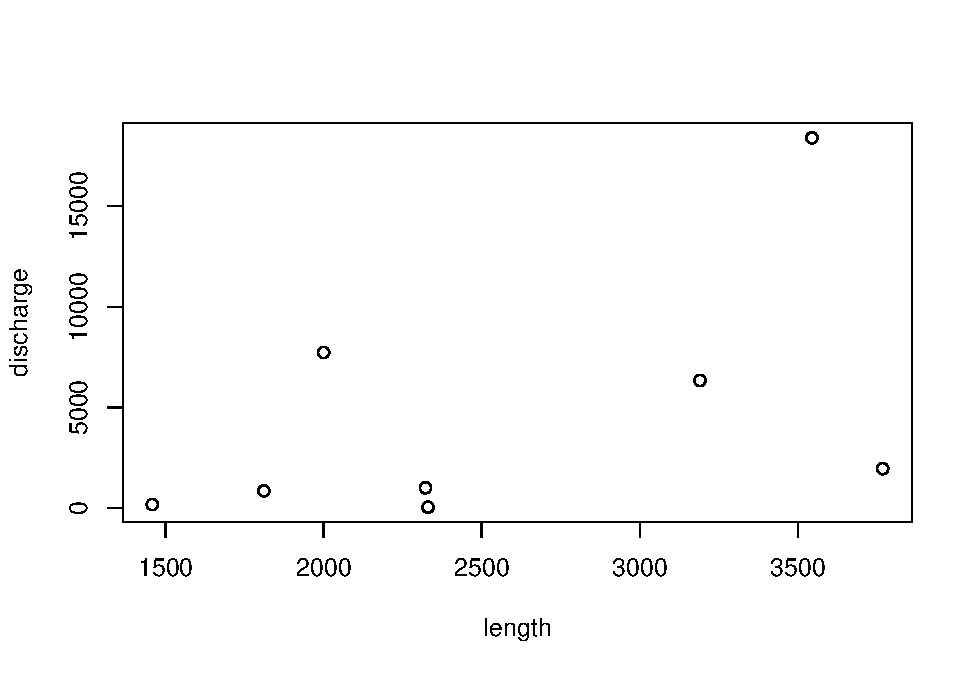
\includegraphics[width=0.75\linewidth]{manuscript_files/figure-latex/rivers-1} 

}

\caption{River length vs discharge}\label{fig:rivers}
\end{figure}

\hypertarget{discussion}{%
\section{Discussion}\label{discussion}}

This is where I talk about my take-home points.

\hypertarget{data-and-code-availability}{%
\section*{Data and Code Availability}\label{data-and-code-availability}}
\addcontentsline{toc}{section}{Data and Code Availability}

The data are available here. The R package are available here. This
article was published using the rticles package \citep{rticles2021}.
Some LaTeX knowledge will be helpful when using rticles.

\bibliographystyle{tfcad}
\bibliography{interactcadsample.bib}


\input{"appendix.tex"}


\end{document}
